\addcontentsline{toc}{chapter}{Appendices}
\chapter{PCA and Canonical Variate}
\label{apx:pcaca}
In this section, two algorithms are developed to recognise human face from the ORL face database. Two algorithms are used to recognise these 40 subjects. One is PCA, another is the canonical variates. The results showed that the canonical variates algorithm has a better performance than PCA on face recognition. 
\section{PCA}
The PCA (principal component analysis), also known as the Karhunen-Loeve transform \cite{Loeve1955}, is a classical method in multivariate statistics. In machine vision, PCA is a good solution for feature selection. The goal of feature selection is to obtain a smaller set of features that accurately represents the original set. The smaller and new set of features will capture as much of original set's variance as possible. Also if a value of one feature can be predicted precisely from the value of the others features, this feature is clearly redundant and needs to be removed. In PCA, the data are taken as points in a very high dimensional space (which is depend on how many features are in the original set), and construct a lower dimensional linear subspace. This subspace describes the main variation of these data points from their mean data point. In other form of explaining PCA, the principle components which are orthogonal to each other from original data, are generated. Each principle component represents one dimension in the original feature space. The original data points can be projected as new points on an axis along this dimension. In this new coordinate, these new points may gather tightly or separate widely, which depends on the principle component chosen. If a few principle components are chosen, that is a few dimensions are chosen, they span a lower dimensional subspace described before as lower dimensional linear subspace. The locations of these new points in the new linear subspace represent the new values of each features selected.

\subsection{Generate Eigenvectors}
The face images in the \mbox{ORL} face database are two-dimensional $92\times 112$ arrays in grey level intensity values. Each image can be considered as a one dimensional array, so that the images become vectors which contain $10304$ digits. Each digit is considered as an feature in the image array. Equivalently, an image becomes a point in $10304$-dimensional space. Obviously, it is a very high dimensional feature space. The very huge space is far more enough describing human face. Therefore, it is possible to reduce the dimensionality of the high dimensional feature space.

The training set of PCA algorithm is the \mbox{ORL} face database. In the database, there are $40$ subjects and each subject has $9$ images. In the training set, there are $M = 360$ face images, and for each image, there are $N=10304$ pixels. Each image is considered as a vector. In the training set, the face images are $\Gamma_1$, $\Gamma_2$, $\ldots$, $\Gamma_M$. The mean face is defined by
\begin{equation}
\Psi = \frac{1}{M}\sum_{n=1}^M \Gamma_n
\end{equation}
The mean face image is shown in \mbox{Figure}.\ref{fig:meanorl}.
\begin{figure}[ht]
 \begin{center}
  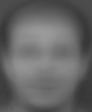
\includegraphics{ch3/figures/mean.jpg}
\caption{The mean face image over $360$ face images in the \mbox{ORL} face database.}
\label{fig:meanorl}
 \end{center}
\end{figure} 
The difference vector describes the degree of each face differs from the mean face by
\begin{equation}
 \Phi_i = \Gamma_i - \Psi
\end{equation}
Here, the covariance matrix of the training set is defined by
\begin{equation}
 C=\frac{1}{M}\sum_{n=1}^M \Phi_n \Phi_n^T
\label{eq:covariancematrix}
\end{equation}
The covariance matrix is a matrix of covariances between features of a vector. It is the natural generalisation to higher dimensions of the concept of the variance. The covariance matrix measures how much two features vary together. If two features tend to vary together (that is, when one of them is above its expected value, then the other features tends to be above its expected value too), then the covariance between the two features will be positive. On the other hand, if one of them is above its expected value and the other feature tends to be below its expected value, then the covariance between the two features will be negative. The covariance matrix $C$ is an $N\times N$ symmetric matrix which characterise the scatter of the training set. A non-zero vector $u$ is an eigenvector of the covariance matrix $C$, if it satisfies the condition:
\begin{equation}
 Cu_k = \nu_k u_k
\end{equation}
where the corresponding eigenvalues are $\nu_k$.

The size of covariance matrix $C$ is $N\times N$ ($N=10304$). It is extremely huge matrix, and the computation cost is tremendous. To reduce the cost, Turk and Pentland’s approach \cite{Turk1991} is adapted to calculate an alternative smaller covariance matrix $L$ rather than original one. In \mbox{Equation} \ref{eq:covariancematrix}, the matrix $C$ can be decomposed as
\begin{equation}
 C = A A^T
\end{equation}
where the matrix $A=[\Phi_1,\ldots,\Phi_M]$. The eigenvector $v_i$ is considered as such that
\begin{equation}
 A^T A v_i = \mu_i v_i
\end{equation}
The both side of the above \mbox{Equation} is pre-multiplied by $A$, then
\begin{equation}
 A A^T A v_i = \mu_i A v_i
\end{equation}
where $Av_i$ is the eigenvector of $C=AA^T$. Following the analysis, an $M\times M$ matrix $L=A^T A$ is constructed. The $M$ eigenvectors $v_i$ of $L$ are found. Therefore, the technique uses a smaller covariance matrix $L$ rather than the original huge matrix $C$. The computation of finding eigenvectors on the original matrix $C$ becomes the computation of finding eigenvectors on the smaller alternative covariance matrix $L$. The size of the matrix is reduced from $N\times N$ to $M\times M$, so that a lot of computational time is saved.

These vectors determine linear combinations of the $M$ training examples to construct the eigenvectors $u_l$
\begin{equation}
 u_l = \sum_{k=1}^M v_{lk} \Phi_k
\end{equation}
Because the size of $L$ is $M\times M$, $M$ eigenvectors can be generated from the technique. With the corresponding eigenvalues, the eigenvectors can be sorted. Each eigenvector $u_l$ is an $N$ length vector. If the eigenvectors are transformed into two-dimensional array with the same size of the images, these arrays display a face-like appearance as ``ghost face''. Hence, these eigenvectors are also called eigenfaces. Some examples of these eigenfaces' are shown in \mbox{Figure} \ref{fig:eigenfaces}.
\begin{figure}[ht]
 \subfigure[1st]{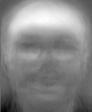
\includegraphics[width=\columnwidth/9]{ch3/figures/eigenface_001.jpg}}
\subfigure[2nd]{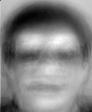
\includegraphics[width=\columnwidth/9]{ch3/figures/eigenface_002.jpg}}
\subfigure[3rd]{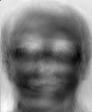
\includegraphics[width=\columnwidth/9]{ch3/figures/eigenface_003.jpg}}
\subfigure[4th]{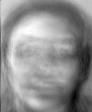
\includegraphics[width=\columnwidth/9]{ch3/figures/eigenface_004.jpg}}
\subfigure[5th]{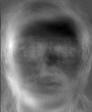
\includegraphics[width=\columnwidth/9]{ch3/figures/eigenface_005.jpg}}
\subfigure[6th]{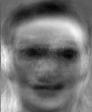
\includegraphics[width=\columnwidth/9]{ch3/figures/eigenface_006.jpg}}
\subfigure[7th]{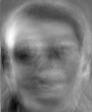
\includegraphics[width=\columnwidth/9]{ch3/figures/eigenface_007.jpg}}
\subfigure[8th]{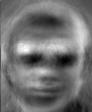
\includegraphics[width=\columnwidth/9]{ch3/figures/eigenface_008.jpg}}
\caption{The top 8 eigenfaces generated from the \mbox{ORL} face database.}
\label{fig:eigenfaces}
\end{figure} 
These eigenfaces are meaningful regarding visual information described in the images. The first eigenface with the biggest corresponding eigenvalue has brighter area across the top of head, which is the area where hair cover. It indicates that in the training set, the variance on the hair area is the most significant. The third eigenface with the third biggest corresponding eigenvalue has two brighter areas locating on the two eyes. It indicates the variance on eyes is significant in the training set.

\subsection{Image Representation}
A face image $\Gamma$ is transformed into its eigenface components (projected into ``face space'') by a simple operation
\begin{equation}
 \omega_k = u_k^T(\Gamma - \Psi)
\end{equation}
where $k=\{1,\ldots,M'\}$ and $M' \le M$. The vector $\Omega = [\omega_1,\ldots,\omega_{M'}]$ that describes the contribution of each eigenface in representing the face image $\Gamma$. The $M'$ eigenfaces are treated as the basis for face images. Hence, an $N$ length image vector is reduced into an $M'$ length vector. The dimensionality has been reduced by choosing $M'$ the number of eigenfaces. The $M'$ eigenfaces span a subspace in which the vector $\Omega$ resides and represents the original image $\Gamma$. In term of face recognition, the subspace is called ``face space'', because all the training examples are face images. The eigenfaces span a lower dimensional subspace which could contains the representations of all possible face images. The vector $\Omega$ is considered as the projection of the $N$-dimensional image space into the $M'$-dimensional face space, so that the features are selected, or the dimensionality is reduced\footnote{In terms of information theory, the image is encoded into $M'$ random variables}.

Each individual face can be represented exactly in terms of a linear combination of the eigenfaces. If the vector $\Omega$ and the eigenfaces are available, the difference between individual one and the mean face is approximately described by
\begin{equation}
 \Phi' = \sum_{i=1}^{M'} \omega_i u_i
\end{equation}
The image $\Gamma'$ can be approximately reconstructed by
\begin{equation}
 \Gamma' = \Phi' + \Psi
\end{equation}
The quality of reconstructed image $\Gamma'$ is controlled by the number of eigenfaces $M'$. Obviously, the more eigenfaces are adopted for the reconstruction, the higher quality of reconstructed image is acquired. The quality of reconstructed image can be modelled by the loss of image energy
\begin{equation}
 \mathrm{Loss} = \frac{\sum_{x,y}\|\Gamma'-\Gamma\|^2}{\sum_{x,y}\|\Gamma\|^2}
\end{equation}
For better reconstructed quality, the loss of image energy should be zero as close as possible. However, there is a trade-off between the higher quality and the more computational cost. 

Therefore, any collection of face images can be approximately reconstructed by storing a small collection $\Omega$ for each face and a small set of eigenfaces. The $\Omega$ describing each face is found by projecting the face image onto each eigenface. In terms of image compression, an image $\Gamma$ can be compressed as $\Gamma'$ with some energy loss.

\subsection{Classification}
The vector $\Omega$ may then be used in a standard pattern recognition algorithm to find predefined face classes, if any, best describes the face. The simplest method for determining which face class provides the best description of an input face image is to find the face class $k$ that minimises the Euclidian distance
\begin{equation}
 \varepsilon_k = \|\Omega-\Omega_k\|^2
\end{equation}
where a vector $\Omega_k$ represents the $k$th face class. The vector is calculated by averaging each individual vector of the eigenface representation within the $k$th face class. A face is classified as belonging to the class $k$ when $\varepsilon_k$ is below some chosen threshold $\theta_k$. Because creating the vector of weights is equivalent to projecting the original face image onto a low-dimensional face space, many images which might look nothing like a face will project onto a given pattern vector. Also the image belonging to the face space is also concerned. The distance between the image and the face space is simply the squared distance between the mean adjusted input image $\Phi$ and $\Phi'$, the reconstructed one. The distance is
\begin{equation}
 \varepsilon^2 = \|\Phi-\Phi' \|^2
\end{equation}
Therefore, for recognising a known individual, calculate the class vector $\Omega_k$ by averaging the eigenface pattern vectors $\Omega$ calculated from the original images of individual. Choose a threshold $\theta_{\varepsilon}$ that defines the maximum allowable distance from any face class, and a threshold that defines the maximum allowable distance from face space. For each new face image to be identified, calculate its pattern vector $\Omega$, the distance $\varepsilon_i$ to each known class, and the distance $\varepsilon$ to face space. If the minimum distance $\varepsilon_k < \theta_{\varepsilon}$ but distance $\varepsilon < \theta_{\varepsilon}$, then the image may be classified as unknown, and optionally used to begin a new face class.

The training set is $360$ images from the \mbox{ORL} face database with $40$ subjects. For each subject, nine images were taken into the training set, and rest one image taken into the testing set. In the testing set, there are $40$ face images and each subject just contains one image. The classifier is the Nearest Neighbour classifier in the PCA implement. The difficulty of PCA is the number of Eigenfaces $M'$. Different number of Eigenfaces gives the different performance on the classification. An exhaustive search on the optimal number of Eigenfaces is given by letting $M'\in\{2,\ldots,220\}$. The performance of classification on different number of Eigenfaces is given in \mbox{Figure} \ref{fig:differenteigens}.
\begin{figure}[ht]
\begin{center}
  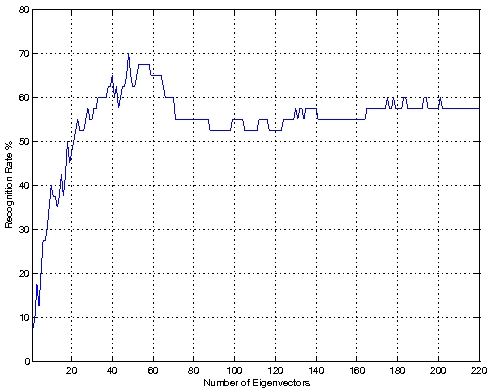
\includegraphics[width=0.7\columnwidth]{ch3/figures/differenteigens.jpg}
\caption{The recognition rates of the PCA approaches with different number of eigenfaces}
\label{fig:differenteigens}
\end{center}
\end{figure} 
The number of eigenfaces is started from $2$ to $220$. From $M'=2$ to $M'=48$, the recognition rate goes up rapidly. When the $M'$ reaches $49$, the recognition rate has its maximum - $70\%$. After the $M'=49$, the recognition rate drops slowly, and converge around $55\%$. It indicates that, in PCA approach on the \mbox{ORL} face database, the optimal number of eigenfaces is $49$, where it achieves the best performance.

\section{Canonical Variate}
PCA yields a set of linear features of a particular dimension that best represents the variance in a high-dimensional dataset. There is no guarantee that this set of features is good for classification. Linear features that emphasise the distinction between classes are known as canonical variates \cite{Forsyth2003}.

To construct canonical variates, assume there are a set of data with $g$ different classes. There are $n_k$ examples in each class, and an example from the $k$th class is $x_{k,i}$, for $i = {1,\ldots,n_k}$. The $j$th class has mean $\mu_j$. It is assumed that there are $p$ features (i.e. that the examples are $p$-dimensional vectors). Write  for the mean of the class means, that is
\begin{equation}
 \bar{\mu} = \frac{1}{g}\sum_{j=1}^{g}\mu_j
\end{equation}
The variance of the class means gives
\begin{equation}
 B=\frac{1}{g-1}\sum_{j=1}^g (\mu_j-\bar{\mu}) (\mu_j-\bar{\mu})^T
\end{equation}
In the simple case, it is assumed that each class has the same covariance, and that this has full rank. It is likely to obtain a set of features where the clusters of examples belonging to a particular class group together tightly, while the discontinuous classes are widely separated. This involves finding a set of features that maximises the ratio of the separation (variance) between the class means to the variance within the class means to the variance within each class. The separation between the class means is typically referred to as \textit{between-class variance}, and the variance within a class is typically referred as \textit{within-class variance}.

The canonical variate approach is concerned on the linear functions of the features as
\begin{equation}
 \upsilon(x) = \nu^T x
\end{equation}
It is likely to maximise the ratio of the between-class variance to the within-class variances for $\nu$. It is assumed that each class has the same covariance $\Sigma$, which is either known or estimated by
\begin{equation}
 \Sigma = \frac{1}{N-1}\sum_{c=1}^g \sum_{i=1}^{n_k} (x_{c,i}-\mu_j) (x_{c,i}-\mu_j)^T
\end{equation}
The total number of examples across all class is $N$. The unit eigenvectors of $\Sigma^{-1}B$ are represented by $\{\nu_1, \nu_2,\ldots,\nu_d\}$. The order of eigenvectors is given by the order of the corresponding eigenvalues, where $\nu_1$ has the largest eigenvalue.  Given a set of features, the projection onto the $k$ eigenvectors spans a $k$-dimensional linear subspace that best separates the class means. The canonical variates are these eigenvectors which can group examples belonging to a particular class together tightly, and widely separate the different classes.

In the experiment of the canonical variates, the \mbox{ORL} face database is adopted. All $400$ images are used to generate the canonical variates. The difficulty of canonical variates is to compute the inverse matrix of the covariance matrix $\Sigma$, because when the data is in a very high dimensional feature space, the covariance matrix is tend to be singular or close to singular. To solve the problem of singular matrix, the size of images is reduce from $92\times 112$ to $18\times 22$. 

From analysis on canonical variates in the \mbox{ORL} face database, the first eigenvector $\nu_1$ (variate) is useless for distinguishing the different classes. The second eigenvector $\nu_2$ displays an excellent performance on classifying the examples. The third eigenvector $\nu_3$ is complex because the covariance matrix is not symmetric. In the third eigenvector, the real part is adopted, but the imaginary part is ignored. With the second eigenvector $\nu_2$ and the real part of the third eigenvector $\Re\{\nu_3\}$, a linear subspace is spanned. In the linear subspace, the $39$ subjects are well separated as \mbox{Figure} \ref{fig:canonicalvariates} shown, which indicates the excellent performance for the canonical variates on classification.
\begin{figure}[ht]
\begin{center}
  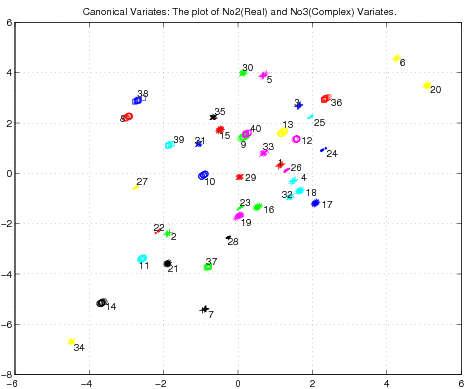
\includegraphics[width=0.9\columnwidth]{ch3/figures/Canonical_Variate_2_3.png}
\label{fig:canonicalvariates}
\caption{The 40 classes of the \mbox{ORL} face database on 2D space constructed by Canonical Variates}
\end{center}
\end{figure} 
